\chapter{Hybrydowy algorytm koordynacji ruchu robotów}

\section{Wprowadzenie} 

Założenia algorytmu

Inspiracja zaczerpnięta z obserwacji grup ludzi i zwierząt oraz ich zachowań.

Wzorce zachowań: 
unikanie kolizji z większym osobnikiem, respekt przed silniejsza grupą.
wprowadzenie zasad społecznych.

Algorytm reaktywny, bezstanowy 

Brak centralnego planowania.

Działający w czasie rzeczywistym.

Koordynacja ruchy robotów inspirowana zjawiskami społecznymi.

Zjawisko respektu przed silniejszym osobnikiem 

Respekt przed liczniejszą grupą.

Reguła podejmowania decyzji w przejściu - priorytetyzowaniu osób wychodzących z pomieszczenia 


Brak jawnej komunikacji 

Algorytm w czasie rzeczywistym adaptuje się do zmieniającego się środowiska.

Omijanie uczestników ruchu stale szukając najlepszej ścieżki do celu.

\section{Zjawisko respektu}

 \begin{itemize}
 \item inspiracje raz jeszcze -- zwierzęta, ale też ludzie, podświadomie unikają konfliktu z "większymi", ale także zakładają, że "mniejsi" ustąpią im z drogi. Nie musi dotyczyć fizycznego rozmiaru, może pozycji w stadzie -- przykład -- wieku --  przykład -- płci -- p - pozycji w hierarchii -... 
 \item grupy -- długi opis - zwierzątka, ludzie -- w grupie raźniej ... 

 \item opis metody -- obliczanie autonomiczne współczynnika na podstawie obserwacji

 \end{itemize}

Algorytm Respektu.

Algorytm obliczania realizujemy według wzoru: 

 \begin{equation}
 k_j = \sum_{i \in R}  \left(   \frac{D_{max} - d_{ij}}{D_{max}} ~ \cdot ~ cos(\phi_{ij}) ~ \cdot f_i \right)
 \label{eq:fearFactor}
 \end{equation}
 \\
 Gdzie:
 \\
 $ k_j $ - współczynnik respektu dla robota $ j $
 \\
 $ d_{ij} $ - odległość pomiędzy robotem $ i $ oraz $ j $
 \\
 $ \phi_{ij} $ - kąt skierowany pomiędzy robotem $ i $ oraz $ j $
 \\
 $ f_i $ - bazowy współczynnik respektu dla robot $ i $
 \\
 $ D_{max} $ - zasięg
 \\
 $ R $ - zbiór robotów
 
 
 \begin{equation}
 \phi_{ij} = \left\{\begin{array}{ll}
 \alpha_i - \alpha_j  & \mbox{jeżeli } ~~~ |\alpha_i - \alpha_j| \leq \frac{\pi}{2} \\
 \frac{\pi}{2} & \mbox{w innym przypadku}
 \cr
 \end{array}\right.
 \label{eq:fearFactorAngle}
 \end{equation}
 
 Gdzie:
 \\
 $ \alpha_i $ - Orientacja $ i $ robota (kąt skierowany),
 \\
 $ \alpha_j $ - Orientacja $ j $ robota (kąt skierowany).
 \\


\section{Zasada priorytetyzowania wychodzących}

Czynnik przejścia

\begin{equation}
p_j = 1 + \psi\left(d_{jl}\right) * \lambda\left(\alpha_j,\gamma_l\right) * \tau \\
\label{eq:factorpassageby}
\end{equation}
\\
\\
\\
Gdzie:
\\
$ p_j $ - Czynnik przejścia przez drzwi dla robota $ j $.
\\
$ \psi\left(d_{jl}\right) $ - Funkcja określająca, w jakim stopniu robot jest w zasięgu działania drzwi.
\\
$ \lambda(\alpha_j,\gamma_l) $ - Funkcja która decyduje, czy robot $j$ wchodzi do pomieszczenia czy wychodzi z niego.
\\
$ \tau \in \mathbb{R}_{+} $ - Współczynnik definiujący wpływ czynnika przejścia na pierwszeństwo. W eksperymentach przyjęliśmy wartość $ \tau = 1 $, ale możliwe jest dynamiczne określanie tego współczynnika na przykład na podstawie stosunku zagęszczeń robotów w sąsiadujących pomieszczeniach.
\\
$ d_{jl} $ - Dystans pomiędzy robotem $ j $ oraz środkiem przejścia (drzwiami) $ l $ (można zmienić na odległość od odcinka stanowiącego drzwi).
\\
$ l $ - Identyfikator drzwi. Lokalizacja drzwi, ich szerokość oraz kierunek otwarcia zdefiniowane zostały w pliku mapy labiryntu i są dostępne dla każdego z robotów.
\\
$ \gamma_l $ - kąt prostopadły do odcinka reprezentującego drzwi, wskazujący kierunek ,,wychodzenia'' przez drzwi. 
\\
%$ v_{j} $ - Prędkość liniowa robota $ j $
\\
\\
\begin{equation}
	\psi\left(d_{jl}\right) = \left\{\begin{array}{ll}
	\frac{R_{l} - d_{jl}}{R_{l}} \mbox{ dla } d_{jl} \le R_{l} \\
		0 \mbox{ w innym przypadku }        
	\cr
	\end{array}\right.
\end{equation}
\\
\noindent
gdzie:\\
$ R_{l} $ - Maksymalny zasięg działania drzwi $l$. 

\begin{equation}
\lambda\left(\alpha_j,\gamma_l\right) = \left\{\begin{array}{ll}
1  \mbox{ dla } - \frac{\pi}{2} \leq \alpha_j - \gamma_l \leq \frac{\pi}{2} \\
0  \mbox{ w innym przypadku }
\cr
\end{array}\right.
\end{equation}


\section{Strefa przejścia}

Integracja 1 i 2 - strefa przejścia 


tu połączymy dwa wzorki w jeden 


\begin{equation}
KP_j = k_j * p_j
\label{eq:fearFactorPS}
\end{equation}


\section{Zasada prawej dłoni}

Algorytm prawej dłoni.

Opis + schemat 

Skąd zaczerpnięto inspiracji

\section{Metoda RVO}

Algorytm RVO - odniesienia do pracy autorów

co to jest.

podać wzór.

krótki opis jak jest to liczone wraz z odniesieniem do literatury.

Informacja o tym że użyliśmy tej metody do wykrywanie kolizji robotów.

\section{Metoda hybrydowa}

Metoda hybrydowa łącząca w jedno koncepcje Respektu czynnika przejścia oraz metody RVO.


Dwie odmiany z czynnikiem przejścia przez drzwi.

\begin{figure}[h]
	\centering
	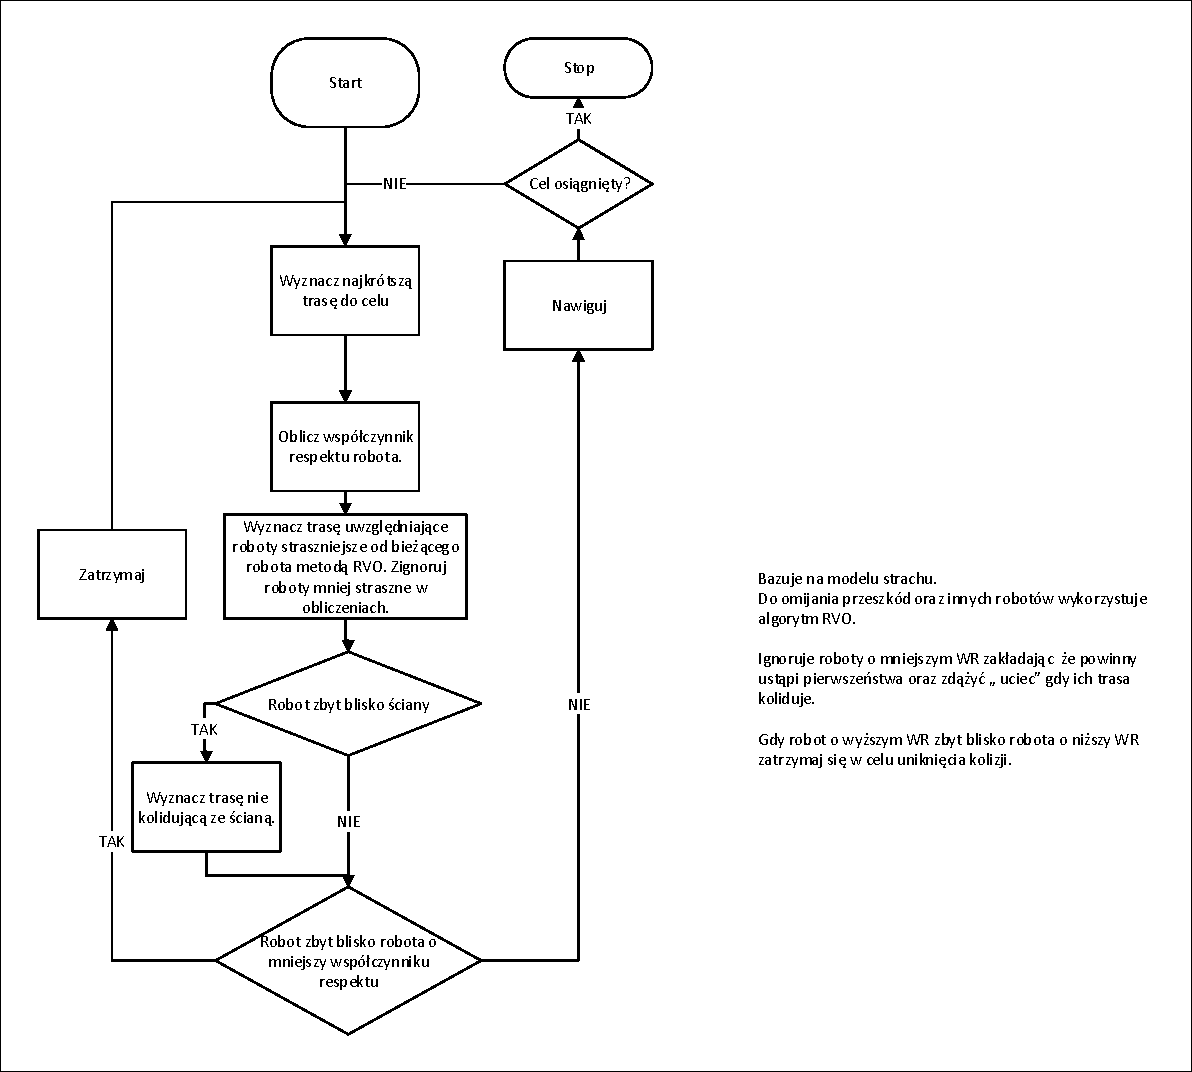
\includegraphics[width=0.45\columnwidth]{img/FearOrginalny.pdf}
	\caption{Hybrydowy algorytm koordynacji ruchu robotów.}
	\label{fig:FearOrginalny}
\end{figure} 

Schemat algorytmu hybrydowego.

\begin{figure}[h]
	\centering
	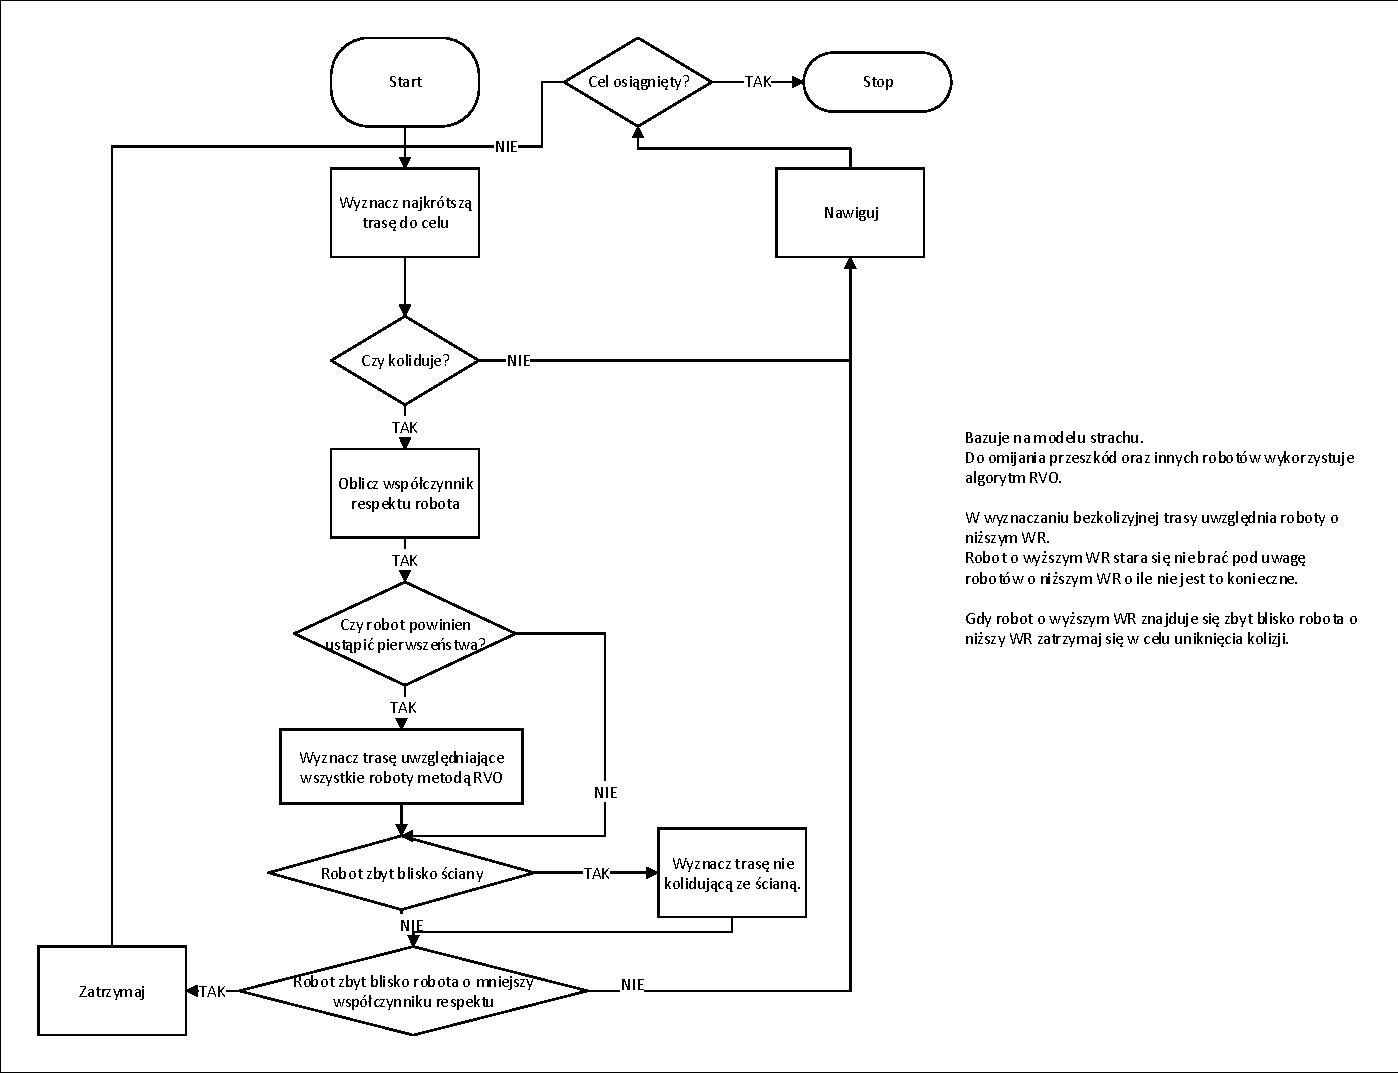
\includegraphics[width=0.45\columnwidth]{img/FearNowy.pdf}
	\caption{Hybrydowy algorytm koordynacji ruchu robotów -  wersja druga.}
	\label{fig:FearNowy}
\end{figure} 


Mutacje algorytmów:
Robot o wyższym WR nie ustępuje pierwszeństwa robotom o z niższymi WR.
Uwzględnianie wszystkich robotów w koordynacji ruchu.

??? Jak nazwać te dwa algorytmy aby w pracy można było je rozróżniać ???
